\section{From real world to 2D images}

Images exist on a 2D plane, whereas the real world is three-dimensional, resulting in a reduction of information compared to the original subject in the real world. 
This reduction is due to the perspective projection, which has the following characteristics:
\begin{itemize}
    \item Nonlinearity.
    \item Lack of shape preservation.
    \item Failure to maintain length ratios.
\end{itemize}
By applying the triangle equality, we can express this perspective projection as:
\[x=f \dfrac{X}{Z} \:\:\:\:\:\: y=f \dfrac{Y}{Z}\]
To mitigate information loss, one approach is to capture an image of a planar scene on a plane that is parallel to the image plane. 
This necessitates that:
\[Z=Z_0=\textnormal{constant}\]
\begin{figure}[H]
    \centering
    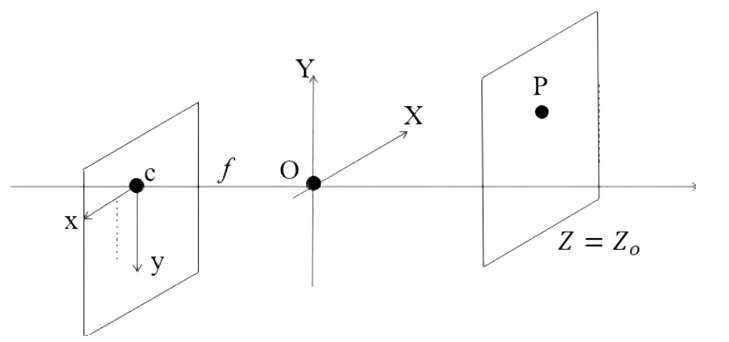
\includegraphics[width=0.5\linewidth]{images/Z0.png}
\end{figure}
In such a scenario, the sole distinction between reality and the projection is a uniform downscaling, while other dimensions are preserved, giving us:
\[x=f \dfrac{X}{Z_0}=kX \:\:\:\:\:\: y=f \dfrac{Y}{Z_0}=kY \]